\chapter{Introduction}\label{chapter:introduction}

Semiconductor lasers present a compact and efficient solid state laser. This type of laser use semiconductor materials as the gain medium. 


Semiconductor lasers are very compact and efficient, and can be mass-produced and integrated with other electronic devices. They have many applications in everyday life and science, such as optical communication, data storage, printing, sensing, medical treatment, and pumping solid-state lasers.

A VECSEL (Vertical-External-Cavity Surface-Emitting Laser) is a type of semiconductor laser that emits light perpendicular to the surface of a semiconductor wafer1. Unlike a VCSEL (Vertical-Cavity Surface-Emitting Laser), which has a closed cavity within the wafer, a VECSEL has an external cavity that is formed by one or more optical elements outside the wafer23. This allows for more flexibility in designing the laser parameters, such as wavelength, output power, beam quality and pulse duration23.

Semiconductor lasers are a type of laser that use semiconductor materials as the gain medium. The gain medium is the part of the laser that amplifies the light by stimulated emission, which is the process of emitting photons with the same energy and phase as the incoming photons. Semiconductor lasers use direct band gap semiconductor materials, which have a small energy difference between the conduction band and the valence band. The conduction band is where electrons can move freely, and the valence band is where electrons are bound to atoms. When an electron jumps from the conduction band to the valence band, it releases a photon with an energy equal to the band gap. This photon can then stimulate another electron to jump and emit another photon, creating a chain reaction of amplification. Semiconductor lasers are very compact and efficient, and can be mass-produced and integrated with other electronic devices. They have many applications in everyday life and science, such as optical communication, data storage, printing, sensing, medical treatment, and pumping solid-state lasers.

Semiconductor lasers were first developed in the early 1960s as homogeneous junction lasers, which were pn junction diodes made on a single material1. The first semiconductor laser was demonstrated by Robert N. Hall and coworkers at the General Electric Research and Development Center in Schenectady, New York, in 19622. Around the same time, two other groups also demonstrated semiconductor lasers independently3. However, these early lasers could only operate at very low temperatures and with high currents, limiting their practical applications.

Since then, semiconductor lasers have undergone significant improvements in performance, efficiency, reliability, and diversity. Some of the key developments include heterojunction lasers, which use different materials for the active region and the cladding layers; quantum well lasers, which confine the electrons and holes in thin layers to enhance the optical gain; distributed feedback lasers, which use a periodic structure to provide wavelength-selective feedback; vertical cavity surface emitting lasers (VCSELs), which emit light perpendicular to the surface of the chip; and quantum cascade lasers, which use intersubband transitions in multiple quantum wells to generate mid-infrared or terahertz radiation.

A VECSEL is a type of semiconductor laser that is based on a VCSEL (Vertical-Cavity Surface-Emitting Laser), but with an external cavity. A VCSEL is a laser diode that emits light perpendicular to the surface of a semiconductor wafer, unlike conventional edge-emitting lasers that emit light from the edges of the wafer12. A VCSEL has a closed cavity within the wafer, which consists of two highly reflective mirrors (called distributed Bragg reflectors) that sandwich a thin layer of active material (called quantum wells) where the light is generated by stimulated emission312.


\section{Gain saturation}

Gain saturation is a phenomenon that occurs when an amplifier device, such as a laser gain medium, cannot maintain a fixed gain for arbitrarily high input powers. This would require adding arbitrary amounts of power to the amplified signal.

For example, a sudden increase in the signal input power of a laser gain medium will reduce the gain only within a certain time because the population in excited laser ions is only reduced with a certain finite rate. This has important consequences for laser dynamics2.

In the steady state (i.e., for long time scales with constant pump power and resonator losses), the gain is where Psat is the saturation power. Note that it has been implicitly assumed that the pump rate is constant, i.e., there are no effects of pump saturation2.

The dynamic behavior of a laser is determined by the interaction of the intracavity light field with the gain medium. Essentially, the intracavity laser power can grow or decay exponentially according to the difference between gain and resonator losses, whereas the rate of change in the gain is determined by stimulated and spontaneous emission (and possibly by other effects such as quenching and energy transfer)3.

In the case of a laser gain medium, the gain does not instantly adjust to the level according to the optical input power because the gain medium stores some amount of energy (excitation energy of the laser-active ions, atoms or molecules), and the stored energy determines the gain. For example, a sudden increase in the signal input power of a laser gain medium will reduce the gain only within a certain time because the population in excited laser ions is only reduced with a certain finite rate. This has important consequences for laser dynamics2.

Gain saturation is a phenomenon that occurs when an amplifier device, such as a laser gain medium, cannot maintain a fixed gain for arbitrarily high input powers. This would require adding arbitrary amounts of power to the amplified signal. Therefore, the gain must be reduced for high input powers; this phenomenon is called gain saturation (or gain compression).

In the case of a laser gain medium, the gain does not instantly adjust to the level according to the optical input power because the gain medium stores some amount of energy (excitation energy of the laser-active ions, atoms or molecules), and the stored energy determines the gain. For example, a sudden increase in the signal input power of a laser gain medium will reduce the gain only within a certain time because the population in excited laser ions is only reduced with a certain finite rate. This has important consequences for laser dynamics.

\begin{figure}[h]
    \centering
    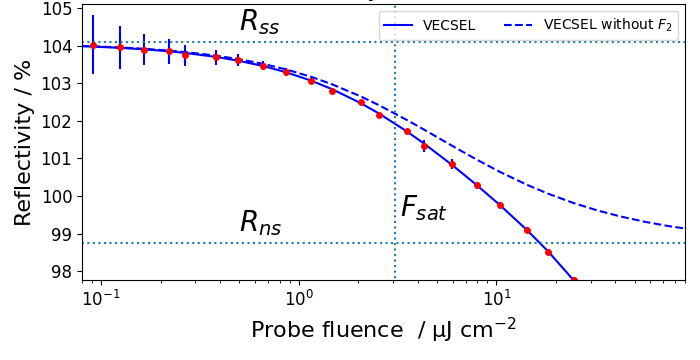
\includegraphics[width=12cm]{images/gainSat.png}
\end{figure}
